\documentclass[1p]{elsarticle_modified}
%\bibliographystyle{elsarticle-num}

%\usepackage[colorlinks]{hyperref}
%\usepackage{abbrmath_seonhwa} %\Abb, \Ascr, \Acal ,\Abf, \Afrak
\usepackage{amsfonts}
\usepackage{amssymb}
\usepackage{amsmath}
\usepackage{amsthm}
\usepackage{scalefnt}
\usepackage{amsbsy}
\usepackage{kotex}
\usepackage{caption}
\usepackage{subfig}
\usepackage{color}
\usepackage{graphicx}
\usepackage{xcolor} %% white, black, red, green, blue, cyan, magenta, yellow
\usepackage{float}
\usepackage{setspace}
\usepackage{hyperref}

\usepackage{tikz}
\usetikzlibrary{arrows}

\usepackage{multirow}
\usepackage{array} % fixed length table
\usepackage{hhline}

%%%%%%%%%%%%%%%%%%%%%
\makeatletter
\renewcommand*\env@matrix[1][\arraystretch]{%
	\edef\arraystretch{#1}%
	\hskip -\arraycolsep
	\let\@ifnextchar\new@ifnextchar
	\array{*\c@MaxMatrixCols c}}
\makeatother %https://tex.stackexchange.com/questions/14071/how-can-i-increase-the-line-spacing-in-a-matrix
%%%%%%%%%%%%%%%

\usepackage[normalem]{ulem}

\newcommand{\msout}[1]{\ifmmode\text{\sout{\ensuremath{#1}}}\else\sout{#1}\fi}
%SOURCE: \msout is \stkout macro in https://tex.stackexchange.com/questions/20609/strikeout-in-math-mode

\newcommand{\cancel}[1]{
	\ifmmode
	{\color{red}\msout{#1}}
	\else
	{\color{red}\sout{#1}}
	\fi
}

\newcommand{\add}[1]{
	{\color{blue}\uwave{#1}}
}

\newcommand{\replace}[2]{
	\ifmmode
	{\color{red}\msout{#1}}{\color{blue}\uwave{#2}}
	\else
	{\color{red}\sout{#1}}{\color{blue}\uwave{#2}}
	\fi
}

\newcommand{\Sol}{\mathcal{S}} %segment
\newcommand{\D}{D} %diagram
\newcommand{\A}{\mathcal{A}} %arc


%%%%%%%%%%%%%%%%%%%%%%%%%%%%%5 test

\def\sl{\operatorname{\textup{SL}}(2,\Cbb)}
\def\psl{\operatorname{\textup{PSL}}(2,\Cbb)}
\def\quan{\mkern 1mu \triangleright \mkern 1mu}

\theoremstyle{definition}
\newtheorem{thm}{Theorem}[section]
\newtheorem{prop}[thm]{Proposition}
\newtheorem{lem}[thm]{Lemma}
\newtheorem{ques}[thm]{Question}
\newtheorem{cor}[thm]{Corollary}
\newtheorem{defn}[thm]{Definition}
\newtheorem{exam}[thm]{Example}
\newtheorem{rmk}[thm]{Remark}
\newtheorem{alg}[thm]{Algorithm}

\newcommand{\I}{\sqrt{-1}}
\begin{document}

%\begin{frontmatter}
%
%\title{Boundary parabolic representations of knots up to 8 crossings}
%
%%% Group authors per affiliation:
%\author{Yunhi Cho} 
%\address{Department of Mathematics, University of Seoul, Seoul, Korea}
%\ead{yhcho@uos.ac.kr}
%
%
%\author{Seonhwa Kim} %\fnref{s_kim}}
%\address{Center for Geometry and Physics, Institute for Basic Science, Pohang, 37673, Korea}
%\ead{ryeona17@ibs.re.kr}
%
%\author{Hyuk Kim}
%\address{Department of Mathematical Sciences, Seoul National University, Seoul 08826, Korea}
%\ead{hyukkim@snu.ac.kr}
%
%\author{Seokbeom Yoon}
%\address{Department of Mathematical Sciences, Seoul National University, Seoul, 08826,  Korea}
%\ead{sbyoon15@snu.ac.kr}
%
%\begin{abstract}
%We find all boundary parabolic representation of knots up to 8 crossings.
%
%\end{abstract}
%\begin{keyword}
%    \MSC[2010] 57M25 
%\end{keyword}
%
%\end{frontmatter}

%\linenumbers
%\tableofcontents
%
\newcommand\colored[1]{\textcolor{white}{\rule[-0.35ex]{0.8em}{1.4ex}}\kern-0.8em\color{red} #1}%
%\newcommand\colored[1]{\textcolor{white}{ #1}\kern-2.17ex	\textcolor{white}{ #1}\kern-1.81ex	\textcolor{white}{ #1}\kern-2.15ex\color{red}#1	}

{\Large $\underline{12a_{1264}~(K12a_{1264})}$}

\setlength{\tabcolsep}{10pt}
\renewcommand{\arraystretch}{1.6}
\vspace{1cm}\begin{tabular}{m{100pt}>{\centering\arraybackslash}m{274pt}}
\multirow{5}{120pt}{
	\centering
	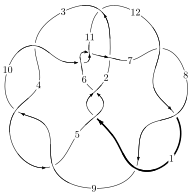
\includegraphics[width=112pt]{../../../GIT/diagram.site/Diagrams/png/2065_12a_1264.png}\\
\ \ \ A knot diagram\footnotemark}&
\allowdisplaybreaks
\textbf{Linearized knot diagam} \\
\cline{2-2}
 &
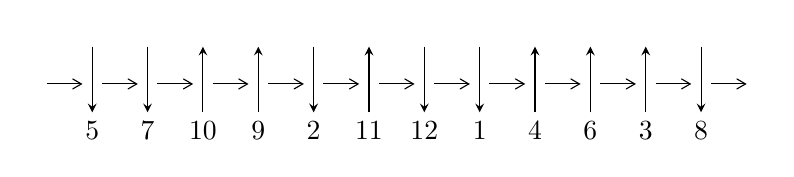
\begin{tikzpicture}[x=20pt, y=17pt]
	% nodes
	\node (C0) at (0, 0) {};
	\node (C1) at (1, 0) {};
	\node (C1U) at (1, +1) {};
	\node (C1D) at (1, -1) {5};

	\node (C2) at (2, 0) {};
	\node (C2U) at (2, +1) {};
	\node (C2D) at (2, -1) {7};

	\node (C3) at (3, 0) {};
	\node (C3U) at (3, +1) {};
	\node (C3D) at (3, -1) {10};

	\node (C4) at (4, 0) {};
	\node (C4U) at (4, +1) {};
	\node (C4D) at (4, -1) {9};

	\node (C5) at (5, 0) {};
	\node (C5U) at (5, +1) {};
	\node (C5D) at (5, -1) {2};

	\node (C6) at (6, 0) {};
	\node (C6U) at (6, +1) {};
	\node (C6D) at (6, -1) {11};

	\node (C7) at (7, 0) {};
	\node (C7U) at (7, +1) {};
	\node (C7D) at (7, -1) {12};

	\node (C8) at (8, 0) {};
	\node (C8U) at (8, +1) {};
	\node (C8D) at (8, -1) {1};

	\node (C9) at (9, 0) {};
	\node (C9U) at (9, +1) {};
	\node (C9D) at (9, -1) {4};

	\node (C10) at (10, 0) {};
	\node (C10U) at (10, +1) {};
	\node (C10D) at (10, -1) {6};

	\node (C11) at (11, 0) {};
	\node (C11U) at (11, +1) {};
	\node (C11D) at (11, -1) {3};

	\node (C12) at (12, 0) {};
	\node (C12U) at (12, +1) {};
	\node (C12D) at (12, -1) {8};
	\node (C13) at (13, 0) {};

	% arrows
	\draw[->,>={angle 60}]
	(C0) edge (C1) (C1) edge (C2) (C2) edge (C3) (C3) edge (C4) (C4) edge (C5) (C5) edge (C6) (C6) edge (C7) (C7) edge (C8) (C8) edge (C9) (C9) edge (C10) (C10) edge (C11) (C11) edge (C12) (C12) edge (C13) ;	\draw[->,>=stealth]
	(C1U) edge (C1D) (C2U) edge (C2D) (C3D) edge (C3U) (C4D) edge (C4U) (C5U) edge (C5D) (C6D) edge (C6U) (C7U) edge (C7D) (C8U) edge (C8D) (C9D) edge (C9U) (C10D) edge (C10U) (C11D) edge (C11U) (C12U) edge (C12D) ;
	\end{tikzpicture} \\
\hhline{~~} \\& 
\textbf{Solving Sequence} \\ \cline{2-2} 
 &
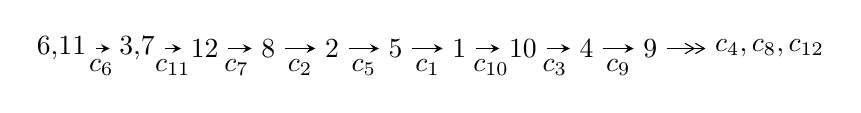
\begin{tikzpicture}[x=23pt, y=7pt]
	% node
	\node (A0) at (-1/8, 0) {6,11};
	\node (A1) at (17/16, 0) {3,7};
	\node (A2) at (17/8, 0) {12};
	\node (A3) at (25/8, 0) {8};
	\node (A4) at (33/8, 0) {2};
	\node (A5) at (41/8, 0) {5};
	\node (A6) at (49/8, 0) {1};
	\node (A7) at (57/8, 0) {10};
	\node (A8) at (65/8, 0) {4};
	\node (A9) at (73/8, 0) {9};
	\node (C1) at (1/2, -1) {$c_{6}$};
	\node (C2) at (13/8, -1) {$c_{11}$};
	\node (C3) at (21/8, -1) {$c_{7}$};
	\node (C4) at (29/8, -1) {$c_{2}$};
	\node (C5) at (37/8, -1) {$c_{5}$};
	\node (C6) at (45/8, -1) {$c_{1}$};
	\node (C7) at (53/8, -1) {$c_{10}$};
	\node (C8) at (61/8, -1) {$c_{3}$};
	\node (C9) at (69/8, -1) {$c_{9}$};
	\node (A10) at (11, 0) {$c_{4},c_{8},c_{12}$};

	% edge
	\draw[->,>=stealth]	
	(A0) edge (A1) (A1) edge (A2) (A2) edge (A3) (A3) edge (A4) (A4) edge (A5) (A5) edge (A6) (A6) edge (A7) (A7) edge (A8) (A8) edge (A9) ;
	\draw[->>,>={angle 60}]	
	(A9) edge (A10);
\end{tikzpicture} \\ 

\end{tabular} \\

\footnotetext{
The image of knot diagram is generated by the software ``\textbf{Draw programme}" developed by Andrew Bartholomew(\url{http://www.layer8.co.uk/maths/draw/index.htm\#Running-draw}), where we modified some parts for our purpose(\url{https://github.com/CATsTAILs/LinksPainter}).
}\phantom \\ \newline 
\centering \textbf{Ideals for irreducible components\footnotemark of $X_{\text{par}}$} 
 
\begin{align*}
I^u_{1}&=\langle 
3.13949\times10^{171} u^{83}-3.46511\times10^{171} u^{82}+\cdots+5.32421\times10^{170} b-1.19378\times10^{171},\\
\phantom{I^u_{1}}&\phantom{= \langle  }-2.38315\times10^{171} u^{83}+3.77864\times10^{171} u^{82}+\cdots+5.32421\times10^{170} a+2.46920\times10^{171},\\
\phantom{I^u_{1}}&\phantom{= \langle  }u^{84}-25 u^{82}+\cdots+13 u-1\rangle \\
I^u_{2}&=\langle 
309 u^{20}-434 u^{19}+\cdots+151 b+4415,\;-1708 u^{20}+524 u^{19}+\cdots+453 a-8666,\\
\phantom{I^u_{2}}&\phantom{= \langle  }u^{21}+u^{20}+\cdots- u+3\rangle \\
\\
\end{align*}
\raggedright * 2 irreducible components of $\dim_{\mathbb{C}}=0$, with total 105 representations.\\
\footnotetext{All coefficients of polynomials are rational numbers. But the coefficients are sometimes approximated in decimal forms when there is not enough margin.}
\newpage
\renewcommand{\arraystretch}{1}
\centering \section*{I. $I^u_{1}= \langle 3.14\times10^{171} u^{83}-3.47\times10^{171} u^{82}+\cdots+5.32\times10^{170} b-1.19\times10^{171},\;-2.38\times10^{171} u^{83}+3.78\times10^{171} u^{82}+\cdots+5.32\times10^{170} a+2.47\times10^{171},\;u^{84}-25 u^{82}+\cdots+13 u-1 \rangle$}
\flushleft \textbf{(i) Arc colorings}\\
\begin{tabular}{m{7pt} m{180pt} m{7pt} m{180pt} }
\flushright $a_{6}=$&$\begin{pmatrix}1\\0\end{pmatrix}$ \\
\flushright $a_{11}=$&$\begin{pmatrix}0\\u\end{pmatrix}$ \\
\flushright $a_{3}=$&$\begin{pmatrix}4.47607 u^{83}-7.09709 u^{82}+\cdots-18.2333 u-4.63769\\-5.89664 u^{83}+6.50822 u^{82}+\cdots-44.1982 u+2.24218\end{pmatrix}$ \\
\flushright $a_{7}=$&$\begin{pmatrix}1\\- u^2\end{pmatrix}$ \\
\flushright $a_{12}=$&$\begin{pmatrix}-18.0492 u^{83}+8.20140 u^{82}+\cdots-415.778 u+31.3112\\2.49929 u^{83}+3.57268 u^{82}+\cdots+164.885 u-10.6843\end{pmatrix}$ \\
\flushright $a_{8}=$&$\begin{pmatrix}15.6145 u^{83}-5.52415 u^{82}+\cdots+412.476 u-26.8042\\3.57130 u^{83}-8.28773 u^{82}+\cdots-88.3591 u+5.88454\end{pmatrix}$ \\
\flushright $a_{2}=$&$\begin{pmatrix}6.88232 u^{83}-8.12828 u^{82}+\cdots+34.3068 u-9.49260\\-5.50421 u^{83}+5.02640 u^{82}+\cdots-60.0099 u+3.27337\end{pmatrix}$ \\
\flushright $a_{5}=$&$\begin{pmatrix}1.92440 u^{83}+5.93603 u^{82}+\cdots+173.361 u-18.2079\\5.97631 u^{83}-8.10078 u^{82}+\cdots+23.9453 u-3.48550\end{pmatrix}$ \\
\flushright $a_{1}=$&$\begin{pmatrix}26.8430 u^{83}-12.5479 u^{82}+\cdots+615.839 u-42.1863\\-6.98242 u^{83}-1.49313 u^{82}+\cdots-279.352 u+19.5683\end{pmatrix}$ \\
\flushright $a_{10}=$&$\begin{pmatrix}- u\\u\end{pmatrix}$ \\
\flushright $a_{4}=$&$\begin{pmatrix}6.30294 u^{83}-9.23048 u^{82}+\cdots-11.9985 u-5.22657\\-7.72350 u^{83}+8.64161 u^{82}+\cdots-50.4330 u+2.83106\end{pmatrix}$ \\
\flushright $a_{9}=$&$\begin{pmatrix}22.0425 u^{83}-15.6464 u^{82}+\cdots+372.604 u-29.2883\\-12.9310 u^{83}+6.98497 u^{82}+\cdots-273.072 u+18.8184\end{pmatrix}$\\&\end{tabular}
\flushleft \textbf{(ii) Obstruction class $= -1$}\\~\\
\flushleft \textbf{(iii) Cusp Shapes $= 24.5986 u^{83}-13.3937 u^{82}+\cdots+525.497 u-43.0239$}\\~\\
\newpage\renewcommand{\arraystretch}{1}
\flushleft \textbf{(iv) u-Polynomials at the component}\newline \\
\begin{tabular}{m{50pt}|m{274pt}}
Crossings & \hspace{64pt}u-Polynomials at each crossing \\
\hline $$\begin{aligned}c_{1},c_{5}\end{aligned}$$&$\begin{aligned}
&u^{84}-2 u^{83}+\cdots+19519 u+2263
\end{aligned}$\\
\hline $$\begin{aligned}c_{2}\end{aligned}$$&$\begin{aligned}
&u^{84}-2 u^{83}+\cdots+160 u+47
\end{aligned}$\\
\hline $$\begin{aligned}c_{3},c_{4},c_{9}\end{aligned}$$&$\begin{aligned}
&u^{84}+u^{83}+\cdots-657 u-23
\end{aligned}$\\
\hline $$\begin{aligned}c_{6},c_{10}\end{aligned}$$&$\begin{aligned}
&u^{84}-25 u^{82}+\cdots+13 u-1
\end{aligned}$\\
\hline $$\begin{aligned}c_{7},c_{8},c_{12}\end{aligned}$$&$\begin{aligned}
&u^{84}-3 u^{83}+\cdots-1131 u-419
\end{aligned}$\\
\hline $$\begin{aligned}c_{11}\end{aligned}$$&$\begin{aligned}
&u^{84}-7 u^{83}+\cdots-210 u-17
\end{aligned}$\\
\hline
\end{tabular}\\~\\
\newpage\renewcommand{\arraystretch}{1}
\flushleft \textbf{(v) Riley Polynomials at the component}\newline \\
\begin{tabular}{m{50pt}|m{274pt}}
Crossings & \hspace{64pt}Riley Polynomials at each crossing \\
\hline $$\begin{aligned}c_{1},c_{5}\end{aligned}$$&$\begin{aligned}
&y^{84}-82 y^{83}+\cdots-175479279 y+5121169
\end{aligned}$\\
\hline $$\begin{aligned}c_{2}\end{aligned}$$&$\begin{aligned}
&y^{84}-14 y^{83}+\cdots-96570 y+2209
\end{aligned}$\\
\hline $$\begin{aligned}c_{3},c_{4},c_{9}\end{aligned}$$&$\begin{aligned}
&y^{84}+95 y^{83}+\cdots-296271 y+529
\end{aligned}$\\
\hline $$\begin{aligned}c_{6},c_{10}\end{aligned}$$&$\begin{aligned}
&y^{84}-50 y^{83}+\cdots-225 y+1
\end{aligned}$\\
\hline $$\begin{aligned}c_{7},c_{8},c_{12}\end{aligned}$$&$\begin{aligned}
&y^{84}-101 y^{83}+\cdots-6461353 y+175561
\end{aligned}$\\
\hline $$\begin{aligned}c_{11}\end{aligned}$$&$\begin{aligned}
&y^{84}+15 y^{83}+\cdots-33050 y+289
\end{aligned}$\\
\hline
\end{tabular}\\~\\
\newpage\flushleft \textbf{(vi) Complex Volumes and Cusp Shapes}
$$\begin{array}{c|c|c}  
\text{Solutions to }I^u_{1}& \I (\text{vol} + \sqrt{-1}CS) & \text{Cusp shape}\\
 \hline 
\begin{aligned}
u &= \phantom{-}0.867430 + 0.455417 I \\
a &= -0.133628 - 0.434117 I \\
b &= \phantom{-}1.36054 + 1.69833 I\end{aligned}
 & -15.6766 + 6.1909 I & \phantom{-0.000000 } 0 \\ \hline\begin{aligned}
u &= \phantom{-}0.867430 - 0.455417 I \\
a &= -0.133628 + 0.434117 I \\
b &= \phantom{-}1.36054 - 1.69833 I\end{aligned}
 & -15.6766 - 6.1909 I & \phantom{-0.000000 } 0 \\ \hline\begin{aligned}
u &= -0.899889 + 0.359409 I \\
a &= -2.37851 - 0.18394 I \\
b &= \phantom{-}2.82048 - 1.30271 I\end{aligned}
 & -14.9740 + 2.0938 I & \phantom{-0.000000 } 0 \\ \hline\begin{aligned}
u &= -0.899889 - 0.359409 I \\
a &= -2.37851 + 0.18394 I \\
b &= \phantom{-}2.82048 + 1.30271 I\end{aligned}
 & -14.9740 - 2.0938 I & \phantom{-0.000000 } 0 \\ \hline\begin{aligned}
u &= -0.868335 + 0.427455 I \\
a &= -0.618033 + 0.133410 I \\
b &= \phantom{-}1.56081 - 1.45456 I\end{aligned}
 & -8.21292 - 3.78416 I & \phantom{-0.000000 } 0 \\ \hline\begin{aligned}
u &= -0.868335 - 0.427455 I \\
a &= -0.618033 - 0.133410 I \\
b &= \phantom{-}1.56081 + 1.45456 I\end{aligned}
 & -8.21292 + 3.78416 I & \phantom{-0.000000 } 0 \\ \hline\begin{aligned}
u &= \phantom{-}0.880746 + 0.388651 I \\
a &= -1.49482 + 0.18154 I \\
b &= \phantom{-}2.15146 + 1.22343 I\end{aligned}
 & -7.93559 + 0.21693 I & \phantom{-0.000000 } 0 \\ \hline\begin{aligned}
u &= \phantom{-}0.880746 - 0.388651 I \\
a &= -1.49482 - 0.18154 I \\
b &= \phantom{-}2.15146 - 1.22343 I\end{aligned}
 & -7.93559 - 0.21693 I & \phantom{-0.000000 } 0 \\ \hline\begin{aligned}
u &= \phantom{-}0.135631 + 0.948644 I \\
a &= -0.890436 - 0.904816 I \\
b &= \phantom{-}0.225715 + 0.006177 I\end{aligned}
 & -11.21050 - 5.58594 I & \phantom{-0.000000 } 0 \\ \hline\begin{aligned}
u &= \phantom{-}0.135631 - 0.948644 I \\
a &= -0.890436 + 0.904816 I \\
b &= \phantom{-}0.225715 - 0.006177 I\end{aligned}
 & -11.21050 + 5.58594 I & \phantom{-0.000000 } 0\\
 \hline 
 \end{array}$$\newpage$$\begin{array}{c|c|c}  
\text{Solutions to }I^u_{1}& \I (\text{vol} + \sqrt{-1}CS) & \text{Cusp shape}\\
 \hline 
\begin{aligned}
u &= -0.175758 + 1.060460 I \\
a &= -0.523782 + 0.447239 I \\
b &= \phantom{-}0.0765748 - 0.0455765 I\end{aligned}
 & -3.42384 + 2.62104 I & \phantom{-0.000000 } 0 \\ \hline\begin{aligned}
u &= -0.175758 - 1.060460 I \\
a &= -0.523782 - 0.447239 I \\
b &= \phantom{-}0.0765748 + 0.0455765 I\end{aligned}
 & -3.42384 - 2.62104 I & \phantom{-0.000000 } 0 \\ \hline\begin{aligned}
u &= \phantom{-}0.916786 + 0.121323 I \\
a &= \phantom{-}0.946036 + 0.576670 I \\
b &= -1.225690 + 0.365216 I\end{aligned}
 & \phantom{-}1.335270 + 0.415812 I & \phantom{-0.000000 } 0 \\ \hline\begin{aligned}
u &= \phantom{-}0.916786 - 0.121323 I \\
a &= \phantom{-}0.946036 - 0.576670 I \\
b &= -1.225690 - 0.365216 I\end{aligned}
 & \phantom{-}1.335270 - 0.415812 I & \phantom{-0.000000 } 0 \\ \hline\begin{aligned}
u &= \phantom{-}1.016070 + 0.378029 I \\
a &= \phantom{-}0.51715 - 1.40535 I \\
b &= -1.15430 + 0.94965 I\end{aligned}
 & -7.39753 + 2.82095 I & \phantom{-0.000000 } 0 \\ \hline\begin{aligned}
u &= \phantom{-}1.016070 - 0.378029 I \\
a &= \phantom{-}0.51715 + 1.40535 I \\
b &= -1.15430 - 0.94965 I\end{aligned}
 & -7.39753 - 2.82095 I & \phantom{-0.000000 } 0 \\ \hline\begin{aligned}
u &= \phantom{-}0.036897 + 0.913172 I \\
a &= -1.140940 - 0.311677 I \\
b &= -0.378045 + 0.235807 I\end{aligned}
 & -5.58935 - 1.48544 I & \phantom{-0.000000 } 0 \\ \hline\begin{aligned}
u &= \phantom{-}0.036897 - 0.913172 I \\
a &= -1.140940 + 0.311677 I \\
b &= -0.378045 - 0.235807 I\end{aligned}
 & -5.58935 + 1.48544 I & \phantom{-0.000000 } 0 \\ \hline\begin{aligned}
u &= -1.079560 + 0.274486 I \\
a &= \phantom{-}0.044313 + 0.682178 I \\
b &= -0.230708 + 0.000959 I\end{aligned}
 & -0.38051 - 2.58331 I & \phantom{-0.000000 } 0 \\ \hline\begin{aligned}
u &= -1.079560 - 0.274486 I \\
a &= \phantom{-}0.044313 - 0.682178 I \\
b &= -0.230708 - 0.000959 I\end{aligned}
 & -0.38051 + 2.58331 I & \phantom{-0.000000 } 0\\
 \hline 
 \end{array}$$\newpage$$\begin{array}{c|c|c}  
\text{Solutions to }I^u_{1}& \I (\text{vol} + \sqrt{-1}CS) & \text{Cusp shape}\\
 \hline 
\begin{aligned}
u &= -0.790280 + 0.392957 I \\
a &= \phantom{-}0.130900 + 0.658695 I \\
b &= \phantom{-}0.429648 - 0.708969 I\end{aligned}
 & -3.37846 + 0.48072 I & \phantom{-0.000000 } 0 \\ \hline\begin{aligned}
u &= -0.790280 - 0.392957 I \\
a &= \phantom{-}0.130900 - 0.658695 I \\
b &= \phantom{-}0.429648 + 0.708969 I\end{aligned}
 & -3.37846 - 0.48072 I & \phantom{-0.000000 } 0 \\ \hline\begin{aligned}
u &= -0.777768 + 0.402665 I \\
a &= \phantom{-}0.36633 - 1.49428 I \\
b &= \phantom{-}0.383311 - 0.248972 I\end{aligned}
 & -8.52352 + 0.24068 I & \phantom{-0.000000 } 0 \\ \hline\begin{aligned}
u &= -0.777768 - 0.402665 I \\
a &= \phantom{-}0.36633 + 1.49428 I \\
b &= \phantom{-}0.383311 + 0.248972 I\end{aligned}
 & -8.52352 - 0.24068 I & \phantom{-0.000000 } 0 \\ \hline\begin{aligned}
u &= \phantom{-}0.760770 + 0.430169 I \\
a &= \phantom{-}0.84316 + 1.22415 I \\
b &= -0.123856 + 0.735006 I\end{aligned}
 & -16.0312 - 2.4553 I & \phantom{-0.000000 } 0 \\ \hline\begin{aligned}
u &= \phantom{-}0.760770 - 0.430169 I \\
a &= \phantom{-}0.84316 - 1.22415 I \\
b &= -0.123856 - 0.735006 I\end{aligned}
 & -16.0312 + 2.4553 I & \phantom{-0.000000 } 0 \\ \hline\begin{aligned}
u &= -1.122160 + 0.152692 I \\
a &= \phantom{-}0.308819 + 0.442069 I \\
b &= -0.549309 + 0.368714 I\end{aligned}
 & -0.34832 - 2.60015 I & \phantom{-0.000000 } 0 \\ \hline\begin{aligned}
u &= -1.122160 - 0.152692 I \\
a &= \phantom{-}0.308819 - 0.442069 I \\
b &= -0.549309 - 0.368714 I\end{aligned}
 & -0.34832 + 2.60015 I & \phantom{-0.000000 } 0 \\ \hline\begin{aligned}
u &= \phantom{-}0.788981 + 0.357640 I \\
a &= -0.34705 + 2.19183 I \\
b &= \phantom{-}1.134540 - 0.534709 I\end{aligned}
 & -8.26520 + 3.03508 I & \phantom{-0.000000 } 0 \\ \hline\begin{aligned}
u &= \phantom{-}0.788981 - 0.357640 I \\
a &= -0.34705 - 2.19183 I \\
b &= \phantom{-}1.134540 + 0.534709 I\end{aligned}
 & -8.26520 - 3.03508 I & \phantom{-0.000000 } 0\\
 \hline 
 \end{array}$$\newpage$$\begin{array}{c|c|c}  
\text{Solutions to }I^u_{1}& \I (\text{vol} + \sqrt{-1}CS) & \text{Cusp shape}\\
 \hline 
\begin{aligned}
u &= -0.790536 + 0.317246 I \\
a &= -0.78228 - 3.05453 I \\
b &= \phantom{-}1.63787 + 1.34551 I\end{aligned}
 & -15.3846 - 5.0998 I & -9.88739 + 7.81278 I \\ \hline\begin{aligned}
u &= -0.790536 - 0.317246 I \\
a &= -0.78228 + 3.05453 I \\
b &= \phantom{-}1.63787 - 1.34551 I\end{aligned}
 & -15.3846 + 5.0998 I & -9.88739 - 7.81278 I \\ \hline\begin{aligned}
u &= -0.814117 + 0.247211 I \\
a &= \phantom{-}1.27667 - 0.87152 I \\
b &= -1.47451 - 0.25088 I\end{aligned}
 & -3.71295 - 3.36373 I & \phantom{-0.000000 } 0 \\ \hline\begin{aligned}
u &= -0.814117 - 0.247211 I \\
a &= \phantom{-}1.27667 + 0.87152 I \\
b &= -1.47451 + 0.25088 I\end{aligned}
 & -3.71295 + 3.36373 I & \phantom{-0.000000 } 0 \\ \hline\begin{aligned}
u &= \phantom{-}0.017616 + 0.849868 I \\
a &= -1.60776 + 0.49117 I \\
b &= -0.293808 - 0.510206 I\end{aligned}
 & -13.28140 + 3.22203 I & -8.45909 + 0. I\phantom{ +0.000000I} \\ \hline\begin{aligned}
u &= \phantom{-}0.017616 - 0.849868 I \\
a &= -1.60776 - 0.49117 I \\
b &= -0.293808 + 0.510206 I\end{aligned}
 & -13.28140 - 3.22203 I & -8.45909 + 0. I\phantom{ +0.000000I} \\ \hline\begin{aligned}
u &= \phantom{-}1.081380 + 0.400450 I \\
a &= -0.633082 - 0.597295 I \\
b &= \phantom{-}1.093700 - 0.167358 I\end{aligned}
 & -0.13372 + 3.12645 I & \phantom{-0.000000 } 0 \\ \hline\begin{aligned}
u &= \phantom{-}1.081380 - 0.400450 I \\
a &= -0.633082 + 0.597295 I \\
b &= \phantom{-}1.093700 + 0.167358 I\end{aligned}
 & -0.13372 - 3.12645 I & \phantom{-0.000000 } 0 \\ \hline\begin{aligned}
u &= \phantom{-}1.131450 + 0.237796 I \\
a &= -0.694414 - 0.201400 I \\
b &= \phantom{-}1.267510 + 0.153739 I\end{aligned}
 & \phantom{-}2.34073 + 0.56455 I & \phantom{-0.000000 } 0 \\ \hline\begin{aligned}
u &= \phantom{-}1.131450 - 0.237796 I \\
a &= -0.694414 + 0.201400 I \\
b &= \phantom{-}1.267510 - 0.153739 I\end{aligned}
 & \phantom{-}2.34073 - 0.56455 I & \phantom{-0.000000 } 0\\
 \hline 
 \end{array}$$\newpage$$\begin{array}{c|c|c}  
\text{Solutions to }I^u_{1}& \I (\text{vol} + \sqrt{-1}CS) & \text{Cusp shape}\\
 \hline 
\begin{aligned}
u &= -1.070570 + 0.439629 I \\
a &= -0.837100 + 0.640723 I \\
b &= \phantom{-}1.57879 + 0.30911 I\end{aligned}
 & -7.50583 - 3.64030 I & \phantom{-0.000000 } 0 \\ \hline\begin{aligned}
u &= -1.070570 - 0.439629 I \\
a &= -0.837100 - 0.640723 I \\
b &= \phantom{-}1.57879 - 0.30911 I\end{aligned}
 & -7.50583 + 3.64030 I & \phantom{-0.000000 } 0 \\ \hline\begin{aligned}
u &= \phantom{-}1.091050 + 0.401626 I \\
a &= -1.36685 - 0.72485 I \\
b &= \phantom{-}1.80488 + 0.99224 I\end{aligned}
 & -2.64462 + 6.21193 I & \phantom{-0.000000 } 0 \\ \hline\begin{aligned}
u &= \phantom{-}1.091050 - 0.401626 I \\
a &= -1.36685 + 0.72485 I \\
b &= \phantom{-}1.80488 - 0.99224 I\end{aligned}
 & -2.64462 - 6.21193 I & \phantom{-0.000000 } 0 \\ \hline\begin{aligned}
u &= -1.119800 + 0.348384 I \\
a &= -1.041310 + 0.452175 I \\
b &= \phantom{-}1.57156 - 0.50425 I\end{aligned}
 & \phantom{-}3.04119 - 3.80641 I & \phantom{-0.000000 } 0 \\ \hline\begin{aligned}
u &= -1.119800 - 0.348384 I \\
a &= -1.041310 - 0.452175 I \\
b &= \phantom{-}1.57156 + 0.50425 I\end{aligned}
 & \phantom{-}3.04119 + 3.80641 I & \phantom{-0.000000 } 0 \\ \hline\begin{aligned}
u &= -0.241783 + 1.214210 I \\
a &= \phantom{-}0.825895 - 0.665293 I \\
b &= \phantom{-}0.430280 + 0.214201 I\end{aligned}
 & -19.1675 + 9.4172 I & \phantom{-0.000000 } 0 \\ \hline\begin{aligned}
u &= -0.241783 - 1.214210 I \\
a &= \phantom{-}0.825895 + 0.665293 I \\
b &= \phantom{-}0.430280 - 0.214201 I\end{aligned}
 & -19.1675 - 9.4172 I & \phantom{-0.000000 } 0 \\ \hline\begin{aligned}
u &= -1.223720 + 0.476158 I \\
a &= \phantom{-}1.47552 - 0.75900 I \\
b &= -1.98062 + 1.83619 I\end{aligned}
 & -9.63548 - 7.89806 I & \phantom{-0.000000 } 0 \\ \hline\begin{aligned}
u &= -1.223720 - 0.476158 I \\
a &= \phantom{-}1.47552 + 0.75900 I \\
b &= -1.98062 - 1.83619 I\end{aligned}
 & -9.63548 + 7.89806 I & \phantom{-0.000000 } 0\\
 \hline 
 \end{array}$$\newpage$$\begin{array}{c|c|c}  
\text{Solutions to }I^u_{1}& \I (\text{vol} + \sqrt{-1}CS) & \text{Cusp shape}\\
 \hline 
\begin{aligned}
u &= \phantom{-}1.215040 + 0.509623 I \\
a &= \phantom{-}1.187300 + 0.462341 I \\
b &= -1.72380 - 1.37434 I\end{aligned}
 & -2.12528 + 6.47250 I & \phantom{-0.000000 } 0 \\ \hline\begin{aligned}
u &= \phantom{-}1.215040 - 0.509623 I \\
a &= \phantom{-}1.187300 - 0.462341 I \\
b &= -1.72380 + 1.37434 I\end{aligned}
 & -2.12528 - 6.47250 I & \phantom{-0.000000 } 0 \\ \hline\begin{aligned}
u &= -1.206440 + 0.592739 I \\
a &= \phantom{-}0.711590 - 0.108206 I \\
b &= -1.32604 + 0.87962 I\end{aligned}
 & -1.89580 - 4.00758 I & \phantom{-0.000000 } 0 \\ \hline\begin{aligned}
u &= -1.206440 - 0.592739 I \\
a &= \phantom{-}0.711590 + 0.108206 I \\
b &= -1.32604 - 0.87962 I\end{aligned}
 & -1.89580 + 4.00758 I & \phantom{-0.000000 } 0 \\ \hline\begin{aligned}
u &= \phantom{-}1.227470 + 0.552497 I \\
a &= \phantom{-}1.011470 + 0.494428 I \\
b &= -1.93617 - 0.69444 I\end{aligned}
 & -7.92021 + 10.93230 I & \phantom{-0.000000 } 0 \\ \hline\begin{aligned}
u &= \phantom{-}1.227470 - 0.552497 I \\
a &= \phantom{-}1.011470 - 0.494428 I \\
b &= -1.93617 + 0.69444 I\end{aligned}
 & -7.92021 - 10.93230 I & \phantom{-0.000000 } 0 \\ \hline\begin{aligned}
u &= -1.220070 + 0.568868 I \\
a &= \phantom{-}0.876785 - 0.353910 I \\
b &= -1.53903 + 0.54048 I\end{aligned}
 & -0.23668 - 8.23782 I & \phantom{-0.000000 } 0 \\ \hline\begin{aligned}
u &= -1.220070 - 0.568868 I \\
a &= \phantom{-}0.876785 + 0.353910 I \\
b &= -1.53903 - 0.54048 I\end{aligned}
 & -0.23668 + 8.23782 I & \phantom{-0.000000 } 0 \\ \hline\begin{aligned}
u &= \phantom{-}1.230280 + 0.643158 I \\
a &= \phantom{-}0.604167 + 0.210222 I \\
b &= -0.894349 - 0.399361 I\end{aligned}
 & \phantom{-}0.72894 + 3.81668 I & \phantom{-0.000000 } 0 \\ \hline\begin{aligned}
u &= \phantom{-}1.230280 - 0.643158 I \\
a &= \phantom{-}0.604167 - 0.210222 I \\
b &= -0.894349 + 0.399361 I\end{aligned}
 & \phantom{-}0.72894 - 3.81668 I & \phantom{-0.000000 } 0\\
 \hline 
 \end{array}$$\newpage$$\begin{array}{c|c|c}  
\text{Solutions to }I^u_{1}& \I (\text{vol} + \sqrt{-1}CS) & \text{Cusp shape}\\
 \hline 
\begin{aligned}
u &= \phantom{-}1.297120 + 0.515464 I \\
a &= \phantom{-}0.116731 + 0.317673 I \\
b &= -0.62017 - 1.29481 I\end{aligned}
 & -9.53768 + 1.73075 I & \phantom{-0.000000 } 0 \\ \hline\begin{aligned}
u &= \phantom{-}1.297120 - 0.515464 I \\
a &= \phantom{-}0.116731 - 0.317673 I \\
b &= -0.62017 + 1.29481 I\end{aligned}
 & -9.53768 - 1.73075 I & \phantom{-0.000000 } 0 \\ \hline\begin{aligned}
u &= \phantom{-}0.573690\phantom{ +0.000000I} \\
a &= \phantom{-}3.04400\phantom{ +0.000000I} \\
b &= -2.22304\phantom{ +0.000000I}\end{aligned}
 & -9.39043\phantom{ +0.000000I} & -12.3580\phantom{ +0.000000I} \\ \hline\begin{aligned}
u &= -0.543911\phantom{ +0.000000I} \\
a &= \phantom{-}1.70271\phantom{ +0.000000I} \\
b &= -1.62590\phantom{ +0.000000I}\end{aligned}
 & -2.29548\phantom{ +0.000000I} & -12.9570\phantom{ +0.000000I} \\ \hline\begin{aligned}
u &= -1.29610 + 0.66766 I \\
a &= -1.121490 + 0.461809 I \\
b &= \phantom{-}1.84156 - 1.37463 I\end{aligned}
 & -15.8625 - 15.9656 I & \phantom{-0.000000 } 0 \\ \hline\begin{aligned}
u &= -1.29610 - 0.66766 I \\
a &= -1.121490 - 0.461809 I \\
b &= \phantom{-}1.84156 + 1.37463 I\end{aligned}
 & -15.8625 + 15.9656 I & \phantom{-0.000000 } 0 \\ \hline\begin{aligned}
u &= \phantom{-}0.254593 + 0.472326 I \\
a &= \phantom{-}1.18965 + 1.73170 I \\
b &= -0.131607 - 0.743334 I\end{aligned}
 & -5.04166 - 2.62453 I & -6.24106 + 4.53514 I \\ \hline\begin{aligned}
u &= \phantom{-}0.254593 - 0.472326 I \\
a &= \phantom{-}1.18965 - 1.73170 I \\
b &= -0.131607 + 0.743334 I\end{aligned}
 & -5.04166 + 2.62453 I & -6.24106 - 4.53514 I \\ \hline\begin{aligned}
u &= \phantom{-}1.29025 + 0.74378 I \\
a &= -0.974417 - 0.227827 I \\
b &= \phantom{-}1.62364 + 1.07684 I\end{aligned}
 & -7.51825 + 11.52590 I & \phantom{-0.000000 } 0 \\ \hline\begin{aligned}
u &= \phantom{-}1.29025 - 0.74378 I \\
a &= -0.974417 + 0.227827 I \\
b &= \phantom{-}1.62364 - 1.07684 I\end{aligned}
 & -7.51825 - 11.52590 I & \phantom{-0.000000 } 0\\
 \hline 
 \end{array}$$\newpage$$\begin{array}{c|c|c}  
\text{Solutions to }I^u_{1}& \I (\text{vol} + \sqrt{-1}CS) & \text{Cusp shape}\\
 \hline 
\begin{aligned}
u &= \phantom{-}0.34130 + 1.50681 I \\
a &= \phantom{-}0.418952 + 0.350787 I \\
b &= \phantom{-}0.551077 - 0.072182 I\end{aligned}
 & -10.54830 - 4.13683 I & \phantom{-0.000000 } 0 \\ \hline\begin{aligned}
u &= \phantom{-}0.34130 - 1.50681 I \\
a &= \phantom{-}0.418952 - 0.350787 I \\
b &= \phantom{-}0.551077 + 0.072182 I\end{aligned}
 & -10.54830 + 4.13683 I & \phantom{-0.000000 } 0 \\ \hline\begin{aligned}
u &= -1.51516 + 0.44607 I \\
a &= -0.120687 - 0.395757 I \\
b &= \phantom{-}0.340696 + 0.691225 I\end{aligned}
 & -6.24520 + 0.56086 I & \phantom{-0.000000 } 0 \\ \hline\begin{aligned}
u &= -1.51516 - 0.44607 I \\
a &= -0.120687 + 0.395757 I \\
b &= \phantom{-}0.340696 - 0.691225 I\end{aligned}
 & -6.24520 - 0.56086 I & \phantom{-0.000000 } 0 \\ \hline\begin{aligned}
u &= \phantom{-}0.411501\phantom{ +0.000000I} \\
a &= -0.200853\phantom{ +0.000000I} \\
b &= -1.42998\phantom{ +0.000000I}\end{aligned}
 & -2.38672\phantom{ +0.000000I} & -9.62140\phantom{ +0.000000I} \\ \hline\begin{aligned}
u &= -0.270452 + 0.276054 I \\
a &= -0.72038 - 1.80958 I \\
b &= -1.46735 + 0.22463 I\end{aligned}
 & -9.67797 + 0.04826 I & -9.15222 + 0.88435 I \\ \hline\begin{aligned}
u &= -0.270452 - 0.276054 I \\
a &= -0.72038 + 1.80958 I \\
b &= -1.46735 - 0.22463 I\end{aligned}
 & -9.67797 - 0.04826 I & -9.15222 - 0.88435 I \\ \hline\begin{aligned}
u &= -1.34711 + 0.90872 I \\
a &= -0.634846 + 0.018768 I \\
b &= \phantom{-}1.19483 - 0.78052 I\end{aligned}
 & -5.98449 - 4.85348 I & \phantom{-0.000000 } 0 \\ \hline\begin{aligned}
u &= -1.34711 - 0.90872 I \\
a &= -0.634846 - 0.018768 I \\
b &= \phantom{-}1.19483 + 0.78052 I\end{aligned}
 & -5.98449 + 4.85348 I & \phantom{-0.000000 } 0 \\ \hline\begin{aligned}
u &= \phantom{-}0.030793 + 0.350452 I \\
a &= \phantom{-}1.22740 - 0.81407 I \\
b &= -0.115966 + 0.287445 I\end{aligned}
 & \phantom{-}0.013893 + 0.880561 I & \phantom{-}0.34073 - 7.72057 I\\
 \hline 
 \end{array}$$\newpage$$\begin{array}{c|c|c}  
\text{Solutions to }I^u_{1}& \I (\text{vol} + \sqrt{-1}CS) & \text{Cusp shape}\\
 \hline 
\begin{aligned}
u &= \phantom{-}0.030793 - 0.350452 I \\
a &= \phantom{-}1.22740 + 0.81407 I \\
b &= -0.115966 - 0.287445 I\end{aligned}
 & \phantom{-}0.013893 - 0.880561 I & \phantom{-}0.34073 + 7.72057 I \\ \hline\begin{aligned}
u &= \phantom{-}0.0693703\phantom{ +0.000000I} \\
a &= -5.36682\phantom{ +0.000000I} \\
b &= -1.15626\phantom{ +0.000000I}\end{aligned}
 & -2.40955\phantom{ +0.000000I} & -6.14340\phantom{ +0.000000I} \\ \hline\begin{aligned}
u &= \phantom{-}1.96261 + 0.71543 I \\
a &= -0.106540 - 0.181324 I \\
b &= \phantom{-}0.303451 + 0.885409 I\end{aligned}
 & -12.62750 - 2.49656 I & \phantom{-0.000000 } 0 \\ \hline\begin{aligned}
u &= \phantom{-}1.96261 - 0.71543 I \\
a &= -0.106540 + 0.181324 I \\
b &= \phantom{-}0.303451 - 0.885409 I\end{aligned}
 & -12.62750 + 2.49656 I & \phantom{-0.000000 } 0\\
 \hline 
 \end{array}$$\newpage\newpage\renewcommand{\arraystretch}{1}
\centering \section*{II. $I^u_{2}= \langle 309 u^{20}-434 u^{19}+\cdots+151 b+4415,\;-1708 u^{20}+524 u^{19}+\cdots+453 a-8666,\;u^{21}+u^{20}+\cdots- u+3 \rangle$}
\flushleft \textbf{(i) Arc colorings}\\
\begin{tabular}{m{7pt} m{180pt} m{7pt} m{180pt} }
\flushright $a_{6}=$&$\begin{pmatrix}1\\0\end{pmatrix}$ \\
\flushright $a_{11}=$&$\begin{pmatrix}0\\u\end{pmatrix}$ \\
\flushright $a_{3}=$&$\begin{pmatrix}3.77042 u^{20}-1.15673 u^{19}+\cdots-30.4812 u+19.1302\\-2.04636 u^{20}+2.87417 u^{19}+\cdots+28.0331 u-29.2384\end{pmatrix}$ \\
\flushright $a_{7}=$&$\begin{pmatrix}1\\- u^2\end{pmatrix}$ \\
\flushright $a_{12}=$&$\begin{pmatrix}-0.697572 u^{20}-3.98234 u^{19}+\cdots+16.0574 u+11.3532\\-2.78808 u^{20}+0.947020 u^{19}+\cdots+7.24503 u-18.6623\end{pmatrix}$ \\
\flushright $a_{8}=$&$\begin{pmatrix}5.23400 u^{20}+3.75717 u^{19}+\cdots-3.54084 u-6.04857\\-9.61589 u^{20}-5.94702 u^{19}+\cdots+43.8411 u-9.35099\end{pmatrix}$ \\
\flushright $a_{2}=$&$\begin{pmatrix}3.32009 u^{20}-0.0905077 u^{19}+\cdots-18.6865 u+4.67329\\-1.97351 u^{20}+2.83444 u^{19}+\cdots+25.1656 u-24.6887\end{pmatrix}$ \\
\flushright $a_{5}=$&$\begin{pmatrix}-4.79029 u^{20}-1.35320 u^{19}+\cdots+20.2561 u-0.203091\\3.06623 u^{20}+0.635762 u^{19}+\cdots-16.8079 u+6.31126\end{pmatrix}$ \\
\flushright $a_{1}=$&$\begin{pmatrix}-0.0794702 u^{20}+2 u^{19}+\cdots-10.2781 u+8.73510\\3.06623 u^{20}-4.36424 u^{19}+\cdots-22.8079 u+25.3113\end{pmatrix}$ \\
\flushright $a_{10}=$&$\begin{pmatrix}- u\\u\end{pmatrix}$ \\
\flushright $a_{4}=$&$\begin{pmatrix}4.55188 u^{20}-1.53422 u^{19}+\cdots-35.6600 u+19.1501\\-2.82781 u^{20}+3.25166 u^{19}+\cdots+33.2119 u-29.2583\end{pmatrix}$ \\
\flushright $a_{9}=$&$\begin{pmatrix}8.29360 u^{20}+6.87638 u^{19}+\cdots-48.9647 u+13.2296\\-0.397351 u^{20}-0.953642 u^{19}+\cdots+14.6689 u+4.03974\end{pmatrix}$\\&\end{tabular}
\flushleft \textbf{(ii) Obstruction class $= 1$}\\~\\
\flushleft \textbf{(iii) Cusp Shapes $= \frac{2196}{151} u^{20}- u^{19}+\cdots-\frac{21155}{151} u+\frac{13662}{151}$}\\~\\
\newpage\renewcommand{\arraystretch}{1}
\flushleft \textbf{(iv) u-Polynomials at the component}\newline \\
\begin{tabular}{m{50pt}|m{274pt}}
Crossings & \hspace{64pt}u-Polynomials at each crossing \\
\hline $$\begin{aligned}c_{1}\end{aligned}$$&$\begin{aligned}
&u^{21}+3 u^{20}+\cdots-3 u-1
\end{aligned}$\\
\hline $$\begin{aligned}c_{2}\end{aligned}$$&$\begin{aligned}
&u^{21}- u^{20}+\cdots+3 u^2+1
\end{aligned}$\\
\hline $$\begin{aligned}c_{3},c_{4}\end{aligned}$$&$\begin{aligned}
&u^{21}+12 u^{19}+\cdots- u+1
\end{aligned}$\\
\hline $$\begin{aligned}c_{5}\end{aligned}$$&$\begin{aligned}
&u^{21}-3 u^{20}+\cdots-3 u+1
\end{aligned}$\\
\hline $$\begin{aligned}c_{6}\end{aligned}$$&$\begin{aligned}
&u^{21}+u^{20}+\cdots- u+3
\end{aligned}$\\
\hline $$\begin{aligned}c_{7},c_{8}\end{aligned}$$&$\begin{aligned}
&u^{21}-14 u^{19}+\cdots- u+1
\end{aligned}$\\
\hline $$\begin{aligned}c_{9}\end{aligned}$$&$\begin{aligned}
&u^{21}+12 u^{19}+\cdots- u-1
\end{aligned}$\\
\hline $$\begin{aligned}c_{10}\end{aligned}$$&$\begin{aligned}
&u^{21}- u^{20}+\cdots- u-3
\end{aligned}$\\
\hline $$\begin{aligned}c_{11}\end{aligned}$$&$\begin{aligned}
&u^{21}+2 u^{19}+\cdots-4 u-1
\end{aligned}$\\
\hline $$\begin{aligned}c_{12}\end{aligned}$$&$\begin{aligned}
&u^{21}-14 u^{19}+\cdots- u-1
\end{aligned}$\\
\hline
\end{tabular}\\~\\
\newpage\renewcommand{\arraystretch}{1}
\flushleft \textbf{(v) Riley Polynomials at the component}\newline \\
\begin{tabular}{m{50pt}|m{274pt}}
Crossings & \hspace{64pt}Riley Polynomials at each crossing \\
\hline $$\begin{aligned}c_{1},c_{5}\end{aligned}$$&$\begin{aligned}
&y^{21}-21 y^{20}+\cdots+11 y-1
\end{aligned}$\\
\hline $$\begin{aligned}c_{2}\end{aligned}$$&$\begin{aligned}
&y^{21}-5 y^{20}+\cdots-6 y-1
\end{aligned}$\\
\hline $$\begin{aligned}c_{3},c_{4},c_{9}\end{aligned}$$&$\begin{aligned}
&y^{21}+24 y^{20}+\cdots-9 y-1
\end{aligned}$\\
\hline $$\begin{aligned}c_{6},c_{10}\end{aligned}$$&$\begin{aligned}
&y^{21}-17 y^{20}+\cdots+121 y-9
\end{aligned}$\\
\hline $$\begin{aligned}c_{7},c_{8},c_{12}\end{aligned}$$&$\begin{aligned}
&y^{21}-28 y^{20}+\cdots+5 y-1
\end{aligned}$\\
\hline $$\begin{aligned}c_{11}\end{aligned}$$&$\begin{aligned}
&y^{21}+4 y^{20}+\cdots+6 y-1
\end{aligned}$\\
\hline
\end{tabular}\\~\\
\newpage\flushleft \textbf{(vi) Complex Volumes and Cusp Shapes}
$$\begin{array}{c|c|c}  
\text{Solutions to }I^u_{2}& \I (\text{vol} + \sqrt{-1}CS) & \text{Cusp shape}\\
 \hline 
\begin{aligned}
u &= -0.382628 + 0.960881 I \\
a &= -0.783937 + 0.776879 I \\
b &= -0.342890 - 0.330936 I\end{aligned}
 & -7.03803 + 1.17985 I & -10.53416 - 1.53522 I \\ \hline\begin{aligned}
u &= -0.382628 - 0.960881 I \\
a &= -0.783937 - 0.776879 I \\
b &= -0.342890 + 0.330936 I\end{aligned}
 & -7.03803 - 1.17985 I & -10.53416 + 1.53522 I \\ \hline\begin{aligned}
u &= \phantom{-}0.982940 + 0.353291 I \\
a &= -1.012910 - 0.905800 I \\
b &= \phantom{-}1.132380 + 0.090306 I\end{aligned}
 & -3.28251 + 4.29159 I & -3.63277 - 6.11599 I \\ \hline\begin{aligned}
u &= \phantom{-}0.982940 - 0.353291 I \\
a &= -1.012910 + 0.905800 I \\
b &= \phantom{-}1.132380 - 0.090306 I\end{aligned}
 & -3.28251 - 4.29159 I & -3.63277 + 6.11599 I \\ \hline\begin{aligned}
u &= \phantom{-}0.708556 + 0.509046 I \\
a &= \phantom{-}0.135333 + 0.600310 I \\
b &= -0.535697 - 0.942644 I\end{aligned}
 & -4.06743 - 0.95196 I & -8.79489 + 1.18736 I \\ \hline\begin{aligned}
u &= \phantom{-}0.708556 - 0.509046 I \\
a &= \phantom{-}0.135333 - 0.600310 I \\
b &= -0.535697 + 0.942644 I\end{aligned}
 & -4.06743 + 0.95196 I & -8.79489 - 1.18736 I \\ \hline\begin{aligned}
u &= -1.091610 + 0.413227 I \\
a &= -0.493026 + 0.465252 I \\
b &= \phantom{-}0.640827 + 0.099354 I\end{aligned}
 & \phantom{-}0.79785 - 2.50319 I & \phantom{-}1.96461 + 1.44745 I \\ \hline\begin{aligned}
u &= -1.091610 - 0.413227 I \\
a &= -0.493026 - 0.465252 I \\
b &= \phantom{-}0.640827 - 0.099354 I\end{aligned}
 & \phantom{-}0.79785 + 2.50319 I & \phantom{-}1.96461 - 1.44745 I \\ \hline\begin{aligned}
u &= \phantom{-}0.806800\phantom{ +0.000000I} \\
a &= \phantom{-}1.75194\phantom{ +0.000000I} \\
b &= -2.80464\phantom{ +0.000000I}\end{aligned}
 & -8.65759\phantom{ +0.000000I} & \phantom{-}0.238680\phantom{ +0.000000I} \\ \hline\begin{aligned}
u &= -0.772407 + 0.123670 I \\
a &= -1.33115 - 2.13554 I \\
b &= \phantom{-}1.95627 + 0.09675 I\end{aligned}
 & -14.9717 - 4.2446 I & -5.10156 + 0.43387 I\\
 \hline 
 \end{array}$$\newpage$$\begin{array}{c|c|c}  
\text{Solutions to }I^u_{2}& \I (\text{vol} + \sqrt{-1}CS) & \text{Cusp shape}\\
 \hline 
\begin{aligned}
u &= -0.772407 - 0.123670 I \\
a &= -1.33115 + 2.13554 I \\
b &= \phantom{-}1.95627 - 0.09675 I\end{aligned}
 & -14.9717 + 4.2446 I & -5.10156 - 0.43387 I \\ \hline\begin{aligned}
u &= -1.117340 + 0.561366 I \\
a &= \phantom{-}1.280040 - 0.423786 I \\
b &= -1.84009 + 1.17636 I\end{aligned}
 & -4.80473 - 6.53656 I & -6.84617 + 5.55680 I \\ \hline\begin{aligned}
u &= -1.117340 - 0.561366 I \\
a &= \phantom{-}1.280040 + 0.423786 I \\
b &= -1.84009 - 1.17636 I\end{aligned}
 & -4.80473 + 6.53656 I & -6.84617 - 5.55680 I \\ \hline\begin{aligned}
u &= \phantom{-}0.659193 + 0.335624 I \\
a &= -0.38753 + 1.68500 I \\
b &= \phantom{-}1.45988 + 0.17681 I\end{aligned}
 & -8.29821 + 2.26290 I & -6.15426 - 0.05048 I \\ \hline\begin{aligned}
u &= \phantom{-}0.659193 - 0.335624 I \\
a &= -0.38753 - 1.68500 I \\
b &= \phantom{-}1.45988 - 0.17681 I\end{aligned}
 & -8.29821 - 2.26290 I & -6.15426 + 0.05048 I \\ \hline\begin{aligned}
u &= -0.667437\phantom{ +0.000000I} \\
a &= \phantom{-}1.11576\phantom{ +0.000000I} \\
b &= -1.90707\phantom{ +0.000000I}\end{aligned}
 & -1.90443\phantom{ +0.000000I} & \phantom{-}10.3540\phantom{ +0.000000I} \\ \hline\begin{aligned}
u &= \phantom{-}1.30830 + 0.61182 I \\
a &= \phantom{-}0.687983 + 0.277223 I \\
b &= -1.18054 - 1.00060 I\end{aligned}
 & -1.78016 + 4.71282 I & -3.94550 - 7.91328 I \\ \hline\begin{aligned}
u &= \phantom{-}1.30830 - 0.61182 I \\
a &= \phantom{-}0.687983 - 0.277223 I \\
b &= -1.18054 + 1.00060 I\end{aligned}
 & -1.78016 - 4.71282 I & -3.94550 + 7.91328 I \\ \hline\begin{aligned}
u &= \phantom{-}1.48798\phantom{ +0.000000I} \\
a &= \phantom{-}0.230450\phantom{ +0.000000I} \\
b &= \phantom{-}0.129677\phantom{ +0.000000I}\end{aligned}
 & -6.38748\phantom{ +0.000000I} & -10.5940\phantom{ +0.000000I} \\ \hline\begin{aligned}
u &= -1.60867 + 0.49513 I \\
a &= -0.310534 + 0.058407 I \\
b &= \phantom{-}0.500870 - 0.950951 I\end{aligned}
 & -12.23280 + 2.44430 I & -1.45463 + 0.34882 I\\
 \hline 
 \end{array}$$\newpage$$\begin{array}{c|c|c}  
\text{Solutions to }I^u_{2}& \I (\text{vol} + \sqrt{-1}CS) & \text{Cusp shape}\\
 \hline 
\begin{aligned}
u &= -1.60867 - 0.49513 I \\
a &= -0.310534 - 0.058407 I \\
b &= \phantom{-}0.500870 + 0.950951 I\end{aligned}
 & -12.23280 - 2.44430 I & -1.45463 - 0.34882 I\\
 \hline 
 \end{array}$$\newpage
\newpage\renewcommand{\arraystretch}{1}
\centering \section*{ III. u-Polynomials}
\begin{tabular}{m{50pt}|m{274pt}}
Crossings & \hspace{64pt}u-Polynomials at each crossing \\
\hline $$\begin{aligned}c_{1}\end{aligned}$$&$\begin{aligned}
&(u^{21}+3 u^{20}+\cdots-3 u-1)(u^{84}-2 u^{83}+\cdots+19519 u+2263)
\end{aligned}$\\
\hline $$\begin{aligned}c_{2}\end{aligned}$$&$\begin{aligned}
&(u^{21}- u^{20}+\cdots+3 u^2+1)(u^{84}-2 u^{83}+\cdots+160 u+47)
\end{aligned}$\\
\hline $$\begin{aligned}c_{3},c_{4}\end{aligned}$$&$\begin{aligned}
&(u^{21}+12 u^{19}+\cdots- u+1)(u^{84}+u^{83}+\cdots-657 u-23)
\end{aligned}$\\
\hline $$\begin{aligned}c_{5}\end{aligned}$$&$\begin{aligned}
&(u^{21}-3 u^{20}+\cdots-3 u+1)(u^{84}-2 u^{83}+\cdots+19519 u+2263)
\end{aligned}$\\
\hline $$\begin{aligned}c_{6}\end{aligned}$$&$\begin{aligned}
&(u^{21}+u^{20}+\cdots- u+3)(u^{84}-25 u^{82}+\cdots+13 u-1)
\end{aligned}$\\
\hline $$\begin{aligned}c_{7},c_{8}\end{aligned}$$&$\begin{aligned}
&(u^{21}-14 u^{19}+\cdots- u+1)(u^{84}-3 u^{83}+\cdots-1131 u-419)
\end{aligned}$\\
\hline $$\begin{aligned}c_{9}\end{aligned}$$&$\begin{aligned}
&(u^{21}+12 u^{19}+\cdots- u-1)(u^{84}+u^{83}+\cdots-657 u-23)
\end{aligned}$\\
\hline $$\begin{aligned}c_{10}\end{aligned}$$&$\begin{aligned}
&(u^{21}- u^{20}+\cdots- u-3)(u^{84}-25 u^{82}+\cdots+13 u-1)
\end{aligned}$\\
\hline $$\begin{aligned}c_{11}\end{aligned}$$&$\begin{aligned}
&(u^{21}+2 u^{19}+\cdots-4 u-1)(u^{84}-7 u^{83}+\cdots-210 u-17)
\end{aligned}$\\
\hline $$\begin{aligned}c_{12}\end{aligned}$$&$\begin{aligned}
&(u^{21}-14 u^{19}+\cdots- u-1)(u^{84}-3 u^{83}+\cdots-1131 u-419)
\end{aligned}$\\
\hline
\end{tabular}\newpage\renewcommand{\arraystretch}{1}
\centering \section*{ IV. Riley Polynomials}
\begin{tabular}{m{50pt}|m{274pt}}
Crossings & \hspace{64pt}Riley Polynomials at each crossing \\
\hline $$\begin{aligned}c_{1},c_{5}\end{aligned}$$&$\begin{aligned}
&(y^{21}-21 y^{20}+\cdots+11 y-1)\\
&\cdot(y^{84}-82 y^{83}+\cdots-175479279 y+5121169)
\end{aligned}$\\
\hline $$\begin{aligned}c_{2}\end{aligned}$$&$\begin{aligned}
&(y^{21}-5 y^{20}+\cdots-6 y-1)(y^{84}-14 y^{83}+\cdots-96570 y+2209)
\end{aligned}$\\
\hline $$\begin{aligned}c_{3},c_{4},c_{9}\end{aligned}$$&$\begin{aligned}
&(y^{21}+24 y^{20}+\cdots-9 y-1)(y^{84}+95 y^{83}+\cdots-296271 y+529)
\end{aligned}$\\
\hline $$\begin{aligned}c_{6},c_{10}\end{aligned}$$&$\begin{aligned}
&(y^{21}-17 y^{20}+\cdots+121 y-9)(y^{84}-50 y^{83}+\cdots-225 y+1)
\end{aligned}$\\
\hline $$\begin{aligned}c_{7},c_{8},c_{12}\end{aligned}$$&$\begin{aligned}
&(y^{21}-28 y^{20}+\cdots+5 y-1)\\
&\cdot(y^{84}-101 y^{83}+\cdots-6461353 y+175561)
\end{aligned}$\\
\hline $$\begin{aligned}c_{11}\end{aligned}$$&$\begin{aligned}
&(y^{21}+4 y^{20}+\cdots+6 y-1)(y^{84}+15 y^{83}+\cdots-33050 y+289)
\end{aligned}$\\
\hline
\end{tabular}
\vskip 2pc
\end{document}